\documentclass[tikz,border=5pt]{standalone}
\usepackage{tikz}
\usetikzlibrary{calc}

\newcommand{\drawCircularSectors}[3]{%
    \pgfmathsetmacro{\n}{0}%
    \foreach \x in {#3} {\pgfmathparse{\n+1}\global\let\n=\pgfmathresult}%
    \pgfmathsetmacro{\anglestep}{360/\n}
    \pgfmathsetmacro{\offset}{\anglestep/2}
    \foreach \i [count=\j] in {#3} {
        \pgfmathsetmacro{\startangle}{90-(\j-1)*\anglestep+\offset}%
        \pgfmathsetmacro{\endangle}{\startangle-\anglestep}%
        \pgfmathsetmacro{\midangle}{\startangle-\anglestep/2}%
        \pgfmathsetmacro{\midradius}{(#1+#2)/2}%
        \fill[blue!20]
            (\startangle:#1)
            arc (\startangle:\endangle:#1)
            -- (\endangle:#2)
            arc (\endangle:\startangle:#2) -- cycle;

        \draw[thick] (\startangle:#1) -- (\startangle:#2);
        \draw[thick] (\endangle:#1) -- (\endangle:#2);
        \node[rotate=\midangle-90] at (\midangle:\midradius) {\i};
    }
    \draw[thick] (0,0) circle (#2);
    \draw[thick] (0,0) circle (#1);
}

\begin{document}

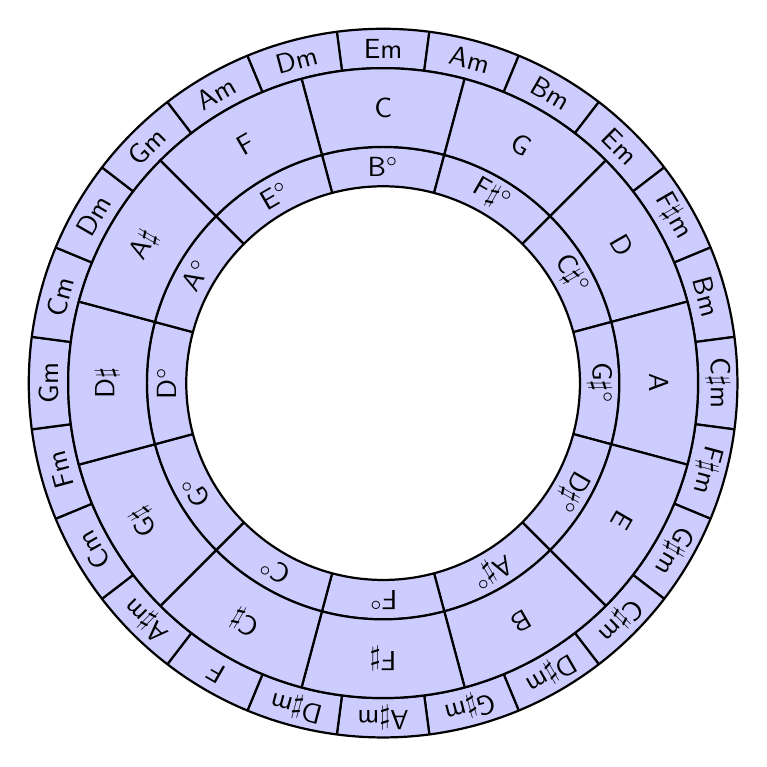
\begin{tikzpicture}[every node/.style={font=\sffamily}]
\drawCircularSectors{4}{4.5}{{Em},{Am},{Bm},{Em},{F$\sharp$m},{Bm},{C$\sharp$m},{F$\sharp$m},{G$\sharp$m},{C$\sharp$m},{D$\sharp$m},{G$\sharp$m},{A$\sharp$m},{D$\sharp$m},{F},{A$\sharp$m},{Cm},{Fm},{Gm},{Cm},{Dm},{Gm},{Am},{Dm}}

\drawCircularSectors{2.5}{3}{{B\textsuperscript{$\circ$}},{F$\sharp$\textsuperscript{$\circ$}},{C$\sharp$\textsuperscript{$\circ$}},{G$\sharp$\textsuperscript{$\circ$}},{D$\sharp$\textsuperscript{$\circ$}},{A$\sharp$\textsuperscript{$\circ$}},{F\textsuperscript{$\circ$}},{C\textsuperscript{$\circ$}},{G\textsuperscript{$\circ$}},{D\textsuperscript{$\circ$}},{A\textsuperscript{$\circ$}},{E\textsuperscript{$\circ$}}}

\drawCircularSectors{3}{4}{{C},{G},{D},{A},{E},{B},{F$\sharp$},{C$\sharp$},{G$\sharp$},{D$\sharp$},{A$\sharp$},{F}}
\end{tikzpicture}

\end{document}
